\section{Greedy Optimization} 

  We have seen that the model space of decision trees was exponential in the number of covariates and number of classes, and super-exponential in the depth. By 1976, it was well known that optimizing a decision tree is NP-complete \cite{1976hyafil}. From an algorithmic point of view, if we have NP-complete problems, the next best thing to do is to look for an \textit{approximate} solution. One way is to simply conduct a greedy search, and this motivated the vast majority of tree algorithms. 

\subsection{Probabilistic Classification Trees} 

  Say that we do a binary split on some covariate $x_i$. This will partition the dataset $\mathcal{D} = \mathcal{D}_1 \sqcup \mathcal{D}_2$. More generally, let's establish the following definition. 

  \begin{definition}[Partition Associated with Node]
    Given a decision tree $\mathcal{T}$ for a dataset $\mathcal{D}$ and any node $t \in \mathcal{T}$, the \textbf{partition of the dataset associated with $t$}, denoted $\mathcal{D}^{[t]}$, is recursively defined as such. 
    \begin{enumerate}
      \item The partition associated with the root node is $\mathcal{D}$, the entire dataset. 
      \item For non-root node $t$, let $t^\prime$ be its parent, which splits on covariate $x_j$ and $t$ filtered with value $x_i = k$. Then, the partition associated with $t$ is 
      \begin{equation}
        \mathcal{D}^{[t]} \coloneqq \{ x^{(i)} \in \mathcal{D}^{[t^\prime]} \mid x^{(i)}_j = k \}
      \end{equation}
    \end{enumerate}
  \end{definition}

  Now if we did not want to split any further, then we would want predict the response for each child node, which are leaves. In classification, the best we can do to minimize our empirical risk is to predict the class $y_1$ that occurs the most frequently in $\mathcal{D}_1$ and $y_2$ for $\mathcal{D}_2$ \hypertarget{frequent}. In regression, we want to predict the average $y_1 = \frac{1}{|\mathcal{D}_1|} \sum_{(x^{(i)}, y^{(i)}) \in \mathcal{D}_1} y^{(i)}$ and $y_2 = \frac{1}{|\mathcal{D}_2|} \sum_{(x^{(i)}, y^{(i)}) \in \mathcal{D}_2} y^{(i)}$. 

  So far, we have not treated classification trees in the probabilistic sense. In each leaf node $l$, there is a hard decision that predicts the value of $y$, say $y = 1$. If we have $K$ classes, then we can also think of each leaf node as a multinomial distribution $p_l$ with all of its mass concentrated at $1$. 

  Now that we have a probabilistic model on each leaf $l$, we can do maximum likelihood estimation of $p_l$ on the partition of the dataset associated with $l$, i.e. $\mathcal{D}_l$. This partition is really the empirical dataset generated by the conditional distribution on the true data generating process $p(y \mid x_{i_1}, \ldots, x_{i_m})$. Now that we have a distribution, our goal is to find a suitable surrogate loss function to minimize. We can do this in two ways. 
  \begin{enumerate}
    \item Maximize likelihood, which will result in us minimizing entropy, or equivalently, maximizing information gain. 
    \item Minimize Gini impurity, which will result in us maximizing Gini reduction. 
  \end{enumerate}
  The Gini reduction method was in fact developed earlier in CART, but since we are more familiar with MLE, let's introduce that first. 

\subsection{ID3 with Information Gain}

  The first way is our familiar friend: MLE. The log-likelihood of this partition under the multinomial $p$ is 
  \begin{equation}
    \log(n!) - \sum_{k=1}^K \log(n_k !) + \sum_{k=1}^K n_k \log(p_k)
  \end{equation}
  were $n = |\mathcal{D}_l|$, $n_k$ is the number of occurrences of a sample of class $k$ in $\mathcal{D}_l$, and $p_k = p(y = k \mid x_{i_1}, \ldots, x_{i_m})$. This with the usual derivations gives our MLE 
  \begin{equation}
    p_k^\ast = \frac{n_k}{n}, \qquad k = 1, \ldots, K
  \end{equation}
  and therefore the value of our loss is the negative log-likelihood with the constant terms removed. 
  \begin{equation}
    \sum_{k=1}^K n_k \log(p_k^\ast)
  \end{equation}
  Scaling down by a constant $n$ doesn't do anything, and we finally get the clean form 
  \begin{equation}
    \sum_{k=1}^K \frac{n_k}{n} \log(p_k^\ast) = \sum_{k=1}^K p_k^\ast \log(p_k^\ast)
  \end{equation}
  which is simply the entropy $H(p^\ast)$! Recall from information theory that this is equivalent to minimizing the KL-divergence between our estimated $p_l$ and the empirical distribution $\mathcal{D}_l$, which is an unbiased estimator of $p(y \mid x_{i_1}, \ldots, x_{i_m})$. 

  Therefore, summing over all leaves, the MLE of our tree $\mathcal{T}$ for a \textit{fixed} structure is the mean of the entropies of each node. 

  \begin{theorem}[Entropy Risk of Classification Tree]
    Given a classification tree $\mathcal{T}$, our expected risk is the expected entropy 
    \begin{equation}
      R(\mathcal{T}) = \mathbb{E}_x \left[ \sum_l H((p^{[l]})^\ast) \cdot \mathbbm{1}(x \in l) \right] = \int \sum_l \left( \sum_{k=1}^K (p_k^{[l]})^\ast \log (p_k^{[l]})^\ast \right) \cdot \mathbbm{1}(x \in l) \,dx 
    \end{equation}
    where $\mathbbm{1}(x \in l)$ is the indicator variable realizing to $1$ if $x$ is generated from the conditional distribution $p^{[l]}$ of leaf node $l$ and $0$ if not. Thus, the empirical risk is 
    \begin{equation}
      \hat{R}(\mathcal{T}) = \frac{1}{n} \sum_{i=1}^n \sum_{l} H( (p^{[l]})^\ast) \cdot \mathbbm{1}(x \in l) = \frac{1}{n} \sum_{i=1}^n \sum_{l} \left( \sum_{k=1}^K (p_k^{[l]})^\ast \log (p_k^{[l]})^\ast \right) \cdot \mathbbm{1}(x \in l)
    \end{equation}
  \end{theorem}

  Essentially, by fixing the structure of the tree, we can---and have---parameterized the leaf nodes with multinomial distributions, which allowed us to calculate the likelihood and even better, a closed form of our MLE. 

  \begin{theorem}[Entropy Risk is Nondecreasing]
    Given two trees $\mathcal{T} \subset \mathcal{T}^\prime$, it is always the case that 
    \begin{equation}
      R(\mathcal{T}^\prime) \leq R(\mathcal{T}), \qquad \hat{R}(\mathcal{T}^\prime) \leq \hat{R}(\mathcal{T}), 
    \end{equation}
  \end{theorem}
  \begin{proof}
    
  \end{proof}

  This loss looks quite complicated, but for greedy algorithms the implementation becomes quite simple. At every step, we are looking for a new split on $\mathcal{T}$ to get $\mathcal{T}^\prime \supset \mathcal{T}$, so from the theorem above, we only need to compute the \textit{Gini reduction}, i.e. the difference in Gini impurities $R(\mathcal{T}) - R(\mathcal{T}^\prime)$. This is only dependent on the node being split, so all we need to do is, for each leaf node, 
  \begin{enumerate}
    \item compute the Gini reduction that splitting on a certain covariate would bring to that node, and then 
    \item multiply it by the probability that a sample will land on that node
  \end{enumerate} 
  This gives the empirical expected Gini reduction of extending $\mathcal{T}$ to $\mathcal{T}^\prime$. 

  \begin{algo}[ID3 Algorithm for Optimizing Classification Tree]
    TBD. Given a single node, we are simply going to label every point to be whatever the majority class is in $\mathcal{D}$. Therefore, we start off with the entropy of our trivial tree $H(Y)$. Then, we want to see which one of the $X_d$ features to split on, and so we can compute the conditional entropy $H(Y, X_d)$ to get the information gain $I(Y; X_d) = H(Y) - H(Y \mid X_d)$ for all $d = 1, \ldots, D$. We want to find a feature $X_d$ that maximize this information gain, i.e. decreases the entropy as much as possible (a greedy algorithm), and we find the next best feature (with or without replacement), so that we have a decreasing sequence. 
    \begin{equation}
      H(X) \geq H(X ; Y) \geq H(X ; Y, Z) \geq H(X ; Y, Z, W) \geq \ldots \geq 0
    \end{equation}
  \end{algo}

  \begin{example}[Crowded Restaurants]
    Continuing the example above, since there are $6$ labels of $0$ and $1$ each, we can model this $Y \sim \mathrm{Bernoulli}(0.5)$ random variable, with entropy 
    \begin{equation}
      H(Y) = \mathbb{E}[-\log_2 p(Y)] = \frac{1}{2} \big( -\log_2 \frac{1}{2} \big) + \frac{1}{2} \big( -\log_2 \frac{1}{2} \big) = 1
    \end{equation}

    Now what would happen if we had branched according to how crowded it was, $X_{\mathrm{crowded}}$. Then, our decision tree would split into 3 sections: 
    \begin{figure}[H]
      \centering 
      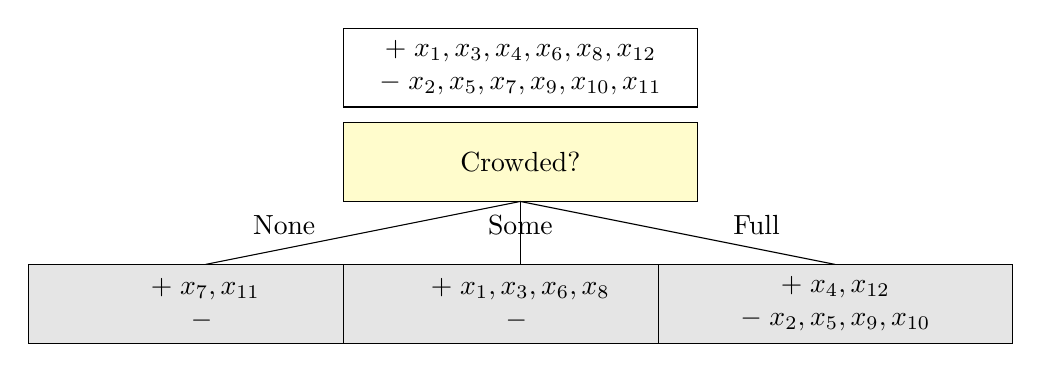
\begin{tikzpicture}[
        box/.style={draw, rectangle, minimum width=4.5cm, minimum height=1cm, align=center},
        yellowbox/.style={box, fill=yellow!20},
        graybox/.style={box, fill=gray!20},
        level 1/.style={sibling distance=6cm},
        level 2/.style={sibling distance=3cm},
        edge from parent/.style={draw, -}
      ]
        % Root node
        \node[box] {$+ \; x_1,x_3,x_4,x_6,x_8,x_{12}$ \\ $- \; x_2,x_5,x_7,x_9,x_{10},x_{11}$};
        \node[yellowbox] at (0,-1.2) {Crowded?};
        
        % Level 1 nodes and edges
        \node[graybox] at (-4,-3) {$+ \; x_7,x_{11}$ \\ $- \; $};
        \node[graybox] at (0,-3) {$+ \; x_1,x_3,x_6,x_8$ \\ $- \; $};
        \node[graybox] at (4,-3) {$+ \; x_4,x_{12}$ \\ $- \; x_2,x_5,x_9,x_{10}$};
        
        % Draw edges
        \draw (0,-1.7) -- (-4,-2.5);
        \draw (0,-1.7) -- (0,-2.5);
        \draw (0,-1.7) -- (4,-2.5);
        
        % Labels for edges
        \node at (-3,-2) {None};
        \node at (0,-2) {Some};
        \node at (3,-2) {Full};
      \end{tikzpicture}
      \caption{Visual of decision tree splitting according to how crowded it is. } 
      \label{fig:crowded_restaurants}
    \end{figure}
    
    In this case, we can define the multinomial distribution $X_{\mathrm{crowded}}$ representing the proportion of the data that is crowded in a specific level. That is, $X_{\mathrm{crowded}} \sim \mathrm{Multinomial}(\frac{2}{12}, \frac{4}{12}, \frac{6}{12} \big)$, with 
    \begin{equation}
      \mathbb{P}(X_{\mathrm{crowded}} = x) = \begin{cases} 2/12 & \text{ if } x = \text{ none} \\ 4/12 & \text{ if } x = \text{ some} \\ 6/12 & \text{ if } x = \text{ full} \end{cases}
    \end{equation}
    Therefore, we can now compute the conditional entropy of this new decision tree conditioned on how crowded the store is 
    \begin{align}
      H(Y \mid X_{\mathrm{crowded}}) & = \sum_x \mathbb{P}(X_{\mathrm{crowded}} = x) H(Y \mid X_{\mathrm{crowded}} = x) \\
      & = \frac{2}{12} H(\mathrm{Bern}(1)) + \frac{4}{12} H(\mathrm{Bern}(0)) + \frac{6}{12} H(\mathrm{Bern}(1/3)) = 0.459 \\
      I(Y; X_{\mathrm{crowded}}) & = 0.541
    \end{align}
    We would do this for all the features and greedily choose the feature that maximizes our information gain. 
  \end{example}

  \begin{example}[Ferrari F1 Race]
    The Ferrari F1 team hired you as a new analyst! You were given the following table of the past race history of the team. You were asked to use information gain to build a decision tree to predict race wins. First, you will need to figure out which feature to split first. 
    \begin{center}
      \begin{tabular}[c]{c|c|c||c}
      Rain & Good Strategy & Qualifying & Win Race \\ \hline
      1 & 0 & 0 & 0 \\
      1 & 0 & 0 & 0 \\
      1 & 0 & 1 & 0 \\
      0 & 0 & 1 & 1 \\
      0 & 0 & 0 & 0 \\
      0 & 1 & 1 & 1 \\
      1 & 0 & 1 & 0 \\
      0 & 1 & 0 & 1 \\
      0 & 0 & 1 & 1 \\
      0 & 0 & 1 & 1 \\
      \end{tabular}
    \end{center}

    Let $X \sim \mathrm{Bernoulli}(1/2)$ be the distribution of whether a car wins a race over the data. Then its entropy is 
    \begin{equation}
      H(X) = \mathbb{E}[-\log_2 p(x)] = \frac{1}{2} \big( -\log_2 \frac{1}{2} \big) + \frac{1}{2} \big( -\log_2 \frac{1}{2} \big) = 1
    \end{equation}

    Let $R \sim \mathrm{Bernoulli}(4/10), G \sim \mathrm{Bernoulli}(2/10), Q \sim \mathrm{Bernoulli}(6/10)$ be the distribution of the features rain, good strategy, and qualifying over the data, respectively. Then, the conditional entropy of $X$ conditioned on each of these random variables is 
    \begin{align*}
      H(X \mid R) & = \mathbb{P}(R = 1)\, H(X \mid R = 1) + \mathbb{P}(R = 0) \, H(X \mid R = 0) \\
      & = \frac{4}{10} \cdot - \big( 1 \cdot \log_2 1 + 0 \cdot \log_2 0 \big) + \frac{6}{10} \cdot - \big( \frac{1}{6} \cdot \log_2 \frac{1}{6} + \frac{5}{6} \cdot \log_2 \frac{5}{6} \big) \approx 0.390 \\
      H(X \mid G) & =  \mathbb{P}(G = 1)\, H(X \mid G = 1) + \mathbb{P}(G = 0) \, H(X \mid G = 0) \\
      & = \frac{2}{10} \cdot - \big( 1 \cdot \log_2 1 + 0 \cdot \log_2 0 \big) + \frac{8}{10} \cdot - \big( \frac{3}{8} \cdot \log_2 \frac{3}{8} + \frac{5}{8} \log_2 \frac{5}{8} \big) \approx 0.763\\
      H(X \mid Q ) & = \mathbb{P}(Q = 1)\, H(X \mid Q = 1) + \mathbb{P}(Q = 0) \, H(X \mid Q = 0) \\
      & = \frac{6}{10} \cdot - \big( \frac{4}{6} \cdot \log_2 \frac{4}{6} + \frac{2}{6} \cdot \log_2 \frac{2}{6} \big) + \frac{4}{10} \cdot - \big( \frac{1}{4} \log_2 \frac{1}{4} + \frac{3}{4} \log_2 \frac{3}{4} \big) \approx 0.875
    \end{align*}

    Therefore, the information gain are 
    \begin{align*}
        I(X; R) & = 1 - 0.390 = 0.610 \\
        I(X; G) & = 1 - 0.763 = 0.237 \\
        I(X; Q) & = 1 - 0.875 = 0.125 
    \end{align*}
    And so I would split on $R$, the rain, which gives the biggest information gain. 
  \end{example}

\subsection{CART with Gini Reduction} 

  The motivation for the Gini impurity is extremely simple. 

  \begin{lemma}[Probability of Lazy Misclassification]
    Given a sample $x \sim \mathrm{Multinomial}(K)$, the probability that one lazily (guessing at random) misclassifies $x$ is 
    \begin{equation}
      1 - \sum_{k=1}^K p_k^2
    \end{equation}
  \end{lemma}
  \begin{proof}
    Let our guess be $y$, which is also an independent uniform multinomial distribution. Given that $x$ is in class $k$, the probability that one misclassifies $x$ is $p(y \neq k \mid x = k) = 1 - p_k$. Therefore, marginalizing over $k$ gives us the total probability of misclassification 
    \begin{align}
      p(y \neq k) & = \sum_{k=1}^K p(y \neq k \mid x = k) p(x = k) \\ 
                  & = \sum_{k=1}^K (1 - p_k) p_k \\ 
                  & = \sum_{k=1}^K p_k - \sum_{k=1}^K p_k^2 \\ 
                  & = 1 - \sum_{k=1}^K p_k^2
    \end{align}
    where I have used the constraint that $\sum_k p_k = 1$. 
  \end{proof}

  Therefore, this gives us a measure of how bad our distribution is to the true one, analogous to the negative log-likelihood. The one major difference is that this is a \textit{pure} impurity score, and the $y$'s are not accounted for here (more on this below). We have the luxury to not account for the $y$'s because we are by default \hyperlink{frequent}{predicting the class that occurs the most frequently in a partition}. 

  \begin{definition}[Gini Impurity]
    The \textbf{Gini impurity} of a $\mathrm{Multinomial}(K)$ random variable with distribution $p$ is 
    \begin{equation}
      G = 1 - \sum_{k=1}^K p_k^2
    \end{equation}
  \end{definition}

  This impurity is something that we want to minimize, and so we can define the expected Gini impurity of our tree as the relevant risk. 

  \begin{theorem}[Gini Risk of Classification Tree]
    Given a classification tree $\mathcal{T}$, the our expected risk is the expected impurity. 
    \begin{equation}
      R(\mathcal{T}) = \mathbb{E}_{x} \left[ \sum_{l \in L} G(p^{[l]}) \cdot \mathbbm{1}(x \in l) \right] = \int \sum_{l \in L} G(p^{[l]}) \cdot \mathbbm{1}(x \in l) \,dx
    \end{equation}
    where $\mathbbm{1}(x \in l)$ is the indicator variable realizing to $1$ if $x$ is generated from the conditional distribution $p^{[l]}$ of leaf node $l$ and $0$ if not. Thus, the empirical risk is 
    \begin{equation}
      \hat{R}(\mathcal{T}) = \frac{1}{n} \sum_{i=1}^n \sum_{l \in L}G(p^{[l]}) \cdot \mathbbm{1}(x^{(i)} \in \mathcal{D}^{[l]})
    \end{equation}
    Note that this does not integrate over the $y$!
  \end{theorem}

  To parse the risk above, consider the following interpretation of the empirical risk. We first sample $x^{(i)}$ from the true distribution. Then, it must belong to exactly one of the conditional distributions (partitions) in the leaf nodes, which is represented by $\mathbbm{1}(x^{(i)} \in l)$, and so the sum $\sum_{l \in L} G(p^{[l]}) \mathbbm{1}(x^{(i)} \in \mathcal{D}^{[l]})$ really boils down to one term: the Gini impurity at the node $l$ that $x$ lands on. Then we average these impurities across $\mathcal{D}$. By marginalizing over the true distribution of $x$ we get the expected risk. 

  \begin{theorem}[Gini Risk is Nondecreasing]
    Given two trees $\mathcal{T} \subset \mathcal{T}^\prime$, it is always the case that 
    \begin{equation}
      R(\mathcal{T}^\prime) \leq R(\mathcal{T}), \qquad \hat{R}(\mathcal{T}^\prime) \leq \hat{R}(\mathcal{T}), 
    \end{equation}
  \end{theorem}

  \begin{example}[Ferrari Example Continued]
    We do the same as the Ferrari example above but now with the Gini reduction. Let $X \sim \mathrm{Bernoulli}(1/2)$ be the distribution of whether a car wins a race over the data. Then its Gini index, which I will label with $\mathcal{G}$, is \[\mathcal{G} (X) = 2 \cdot \frac{1}{2} \cdot \frac{1}{2} = \frac{1}{2}\]
    Let $R \sim \mathrm{Bernoulli}(4/10), G \sim \mathrm{Bernoulli}(2/10), Q \sim \mathrm{Bernoulli}(6/10)$ be the distribution of the features rain, good strategy, and qualifying over the data, respectively. Then we compute the conditional expectation 
    \begin{align*}
        \mathbb{E}[\mathcal{G}(X \mid R)] & = \mathbb{P}(R = 1)\, \mathcal{G}(X \mid R = 1) + \mathbb{P}(R = 0) \, \mathcal{G}(X \mid R = 0) \\ 
        & = \frac{4}{10} \bigg[ 2 \cdot \frac{4}{4} \cdot \frac{0}{4} \bigg] + \frac{6}{10} \bigg[ 2 \cdot \frac{1}{6} \cdot \frac{5}{6} \bigg] \approx 0.167 \\
        \mathbb{E}[\mathcal{G}(X \mid G)] & = \mathbb{P}(G = 1)\, \mathcal{G}(X \mid G = 1) + \mathbb{P}(G = 0) \, \mathcal{G}(X \mid G = 0) \\ 
        & = \frac{2}{10} \bigg[ 2 \cdot \frac{2}{2} \cdot \frac{0}{2} \bigg] + \frac{8}{10} \bigg[ 2 \cdot \frac{3}{8} \cdot \frac{5}{8} \bigg] \approx 0.375 \\
        \mathbb{E}[\mathcal{G}(X \mid Q)] & = \mathbb{P}(Q = 1)\, \mathcal{G}(X \mid Q = 1) + \mathbb{P}(Q = 0) \, \mathcal{G}(X \mid Q = 0) \\ 
        & = \frac{6}{10} \bigg[ 2 \cdot \frac{4}{6} \cdot \frac{2}{6} \bigg] + \frac{4}{10} \bigg[ 2 \cdot \frac{1}{4} \cdot \frac{3}{4} \bigg] \approx 0.417
    \end{align*}
    Therefore, the Gini reduction, which I'll denote as $I_{\mathcal{G}}$, is 
    \begin{align*}
        I_{\mathcal{G}} (X ; R) & = 0.5 - 0.167 = 0.333 \\
        I_{\mathcal{G}} (X ; G) & = 0.5 - 0.375 = 0.125 \\
        I_{\mathcal{G}} (X ; Q) & = 0.5 - 0.417 = 0.083
    \end{align*}
    Since branching across the feature $R$, the rain, gives the biggest Gini reduction, we want to split on the rain feature first. 
  \end{example}

\subsection{c4.5} 
